\section{Discussion}

\subsection{Time constraints}
In our project we were trying to explore as many valid options for classifiers as it was feasible possible. We ended up exploring more than 10 different algorithms to predict sentiment. While we did not achieve great results with most of them, this is not an indication of the algorithms not performing well to our task, as the reason could purely be how we allocated our time. Initially, we tested the base configurations of many of the different technologies and went with the ones we achieved the best results with - the SVM variations. As described in section \ref{MML} about MML, we quickly abandoned the framework, but as clearly seen in section \ref{analysis}, the framework ended up up achieving the third best result only with use of the base configuration and the entirety of out dataset, and had we spend enough time on it, we possibly could have improved it further. 

\subsection{Negatives and Neutrals}
Throughout the project it was quite clear to us that we had issues distinguishing negatives from neutrals and vice-versa. Firstly, if we purely tried to classify positives and not positives, we would achieve	around 87\% accuracy, which clearly indicates that we had no real issue with predicting the positive sentimentet comments. While this can be because positive sentences in general are more unique	
, we can definitely say that the problem with inaccuracies was not due to classifying positives.	

We have two ideas as to why we had issues with differentiating the classes:	
One of the reasons might be that even though we became more reliable in annotating the data after establishing guide lines, it became evident in our cross-validation of the data that most of the discrepancies were neutral/negatives. An example of this confusion becomes quite clear in the following sentence: "De holdt mig mange gange i fængsel". This sentence was annotated as -1, but the sentence is not inherently negative og positive, because it is only stating a fact. Therefore it was changed to 0.

The other reason might be that negative and neutral sentences are inherently much a like, and in many cases what really differentiates them are the tone, which an algorithm will find very difficult to determine without a large quantity of data. An example of this is a sentence like: "hvorfor så ikke denne dag der skulle kun stemmes og babyen kan helt sikkert ikke røbe noget af resultaterne" where to a human it does not really make sense hence we feel it is neutral. We can't predict the sentiment and thus find it neutral, but the classifiers predict it to be -1. As also seen below in figure \ref{negandneu}, our SVM classifier had mostly difficulties differentiating these two classes.

With more data, it might be possible for the SVM to better tell them apart, which brings us to the next section.
\begin{figure}[H]
	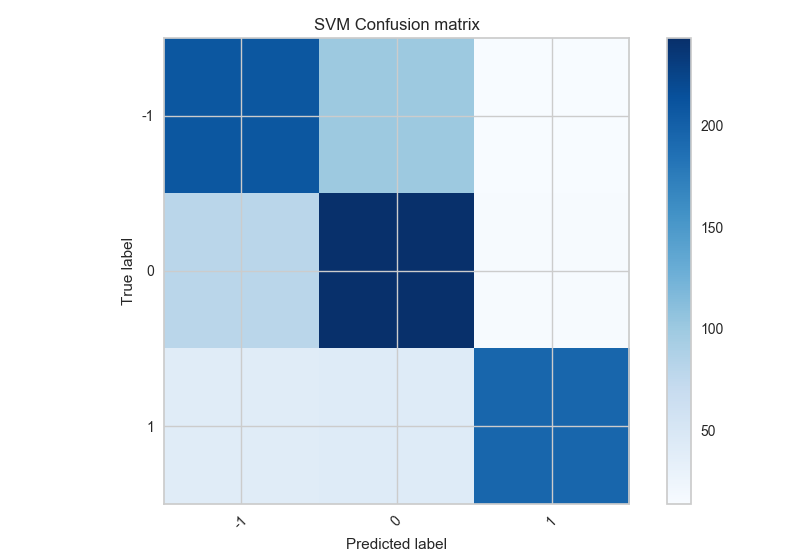
\includegraphics[width=8cm]{Images/ConfusionMatrixThreeClassesSVM}
	\caption{Confusion Matrix on our SVM.}
	\label{negandneu}
\end{figure}


\subsection{Accuracy and Diversity} \label{learningcurve}
One of the reasons we believe that we are not achieving a higher accuracy is that we did not fulfil our goal of creating a diverse dataset; in fact, we unfortunately might have created a much too narrow scope. We believe this to be a flaw in our methodology in which we did not focus on diversifying the articles we collected data from. Instead, we were focused on finding articles with many comments in the belief that there would be a lot more data to collect. A prime example of this is that one of our group members collected 2500 sentences from only 18 articles. This means that 27,75\% of our dataset originates from only 7,53\% of the different articles. Another reason we assume to be a causation for a lower accuracy can be seen from the following graphs.

\begin{figure}[H]
	\centering
	\subfloat[Learning curve with word. \label{lcword}]{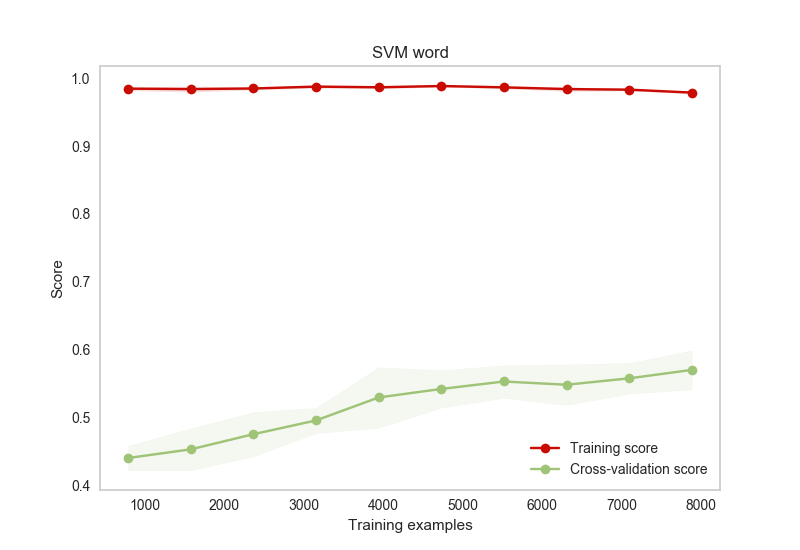
\includegraphics[width=.5\linewidth]{Images/LearningCurveWord}}
	\subfloat[Learning curve with char\_wb.\label{lccharwb}]{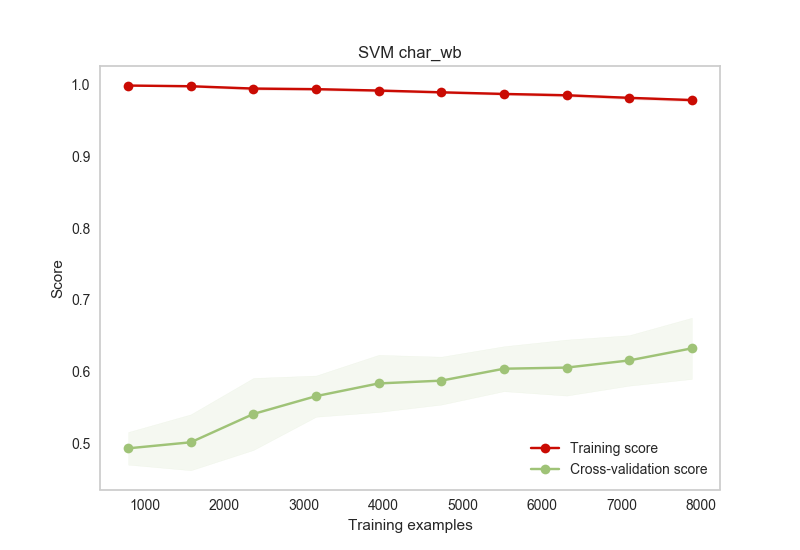
\includegraphics[width=.5\linewidth]{Images/LearningCurveCharWB}
	}
	\caption{Graphs of both learning curves for our SVM.}
\end{figure}

The graphs in figure \ref{lcword} and \ref{lccharwb} shows how the average accuracy of our cross validation iterations increase with the amount of data samples we give it. As sklearns user guide to learning curves states \cite{learningcurve}: \textit{If the training score is much greater than the validation score for the maximum number of training samples, adding more training samples will most likely increase generalization.}.
Since our training score is largely stable and our cross validation score is increasing, it could imply that we do not have enough data, and with that, not enough features.

\begin{figure}[H]
    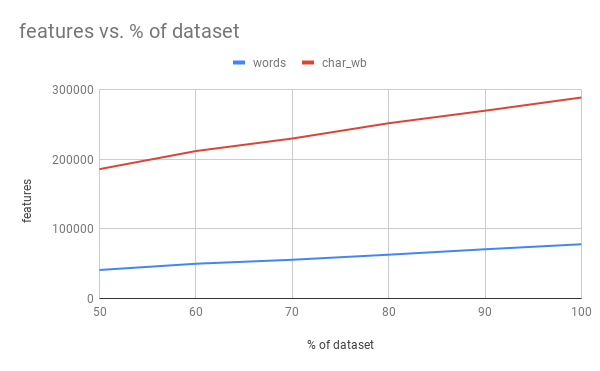
\includegraphics[width=8cm]{Images/DatasetFeatures}
    \centering
    \caption{Feature space showcase of our SVM}
    \label{featspace}
\end{figure}
As seen in figure \ref{featspace}, we can see that both when tokenizing words and characters, our feature space continues to increase linearly with the amount of training samples we have. The problem with increasing the feature space is the \textit{curse of dimensionality}. The curse of dimensionality says that the more features or dimensions we have, the more data we need to generalize accurately grows exponentially. That is, the more dimensions we have, the longer it will take to train, and the more memory it will use.

To sum it up we have some indications that our dataset is not entirely representative for comments on political articles on social media. To disproof our hypothesis we did an experiment, where we collected 100 completely random, unseen and from a very broad spectrum of media/articles sentences. We then trained our SVM with randomly selected 90\% of the dataset and then 100\%. Firstly, we did the the version with 90\%, because all the other versions of our SVM, MML and NN had 10\% of the dataset as test data. Secondly, we did a 100\% version to test how our SVM would perform in the real world, but it would also be able to provide us with indications of whether or not our hypothesis about the lack of data was correct. 

As seen in figure \ref{shit} our accuracy mean clearly falls with 3\% in the 90\% version, when we use sentences that were touching political topics, we had not previously seen before. This is an indication of our hypothesis about a flaw in the methodology being correct. This is easily solved by increasing the amount of data and making sure in the future that the data is more diverse. What we can see with the 100\% version is that the accuracy increases on the 100 samples, which again is an indication of our hypothesis that we are lacking data has merit. Also, as seen in \ref{learningcurve}, increasing the amount of data is still indirectly increasing the diversity of the dataset.

\begin{table}[H]
	\begin{tabular}{@{}lll@{}}
		\toprule
		& Accuracy  & F1 Score \\ \midrule
		90\%  & 63.7255\% & 0.6340   \\
		100\% & 62.4709\% & 0.6218   \\ \bottomrule
	\end{tabular}
	\centering
	\caption{Results of 100 unique sentences}
	\label{shit}
\end{table}



